% This example is meant to be compiled with lualatex or xelatex

% The theme itself also supports pdflatex
\PassOptionsToPackage{unicode}{hyperref}
\documentclass[aspectratio=1610, 10pt]{beamer}

% Load packages you need here
\usepackage{polyglossia}
\setmainlanguage{english}
\usepackage[font=small,labelfont=bf]{caption}
\usepackage{csquotes}
\usepackage{siunitx}
\usepackage{subfigure}

\usepackage{amsmath}
\usepackage{amssymb}
\usepackage{mathtools}

\usepackage{hyperref}
\usepackage{bookmark}
\usepackage[absolute,overlay]{textpos}

%\usepackage[texcoord,
%grid,gridcolor=red!10,subgridcolor=green!10,gridunit=pt]
%{eso-pic}
% load the theme after all packages

\usetheme[
  showtotalframes, % show total number of frames in the footline
]{tudo}

% Put settings here, like
\unimathsetup{
  math-style=ISO,
  bold-style=ISO,
  nabla=upright,
  partial=upright,
  mathrm=sym,
}

\title{\Large{Cherenkov Detectors}}
\author[C.~Krause]{\normalsize{Christopher Krause}}
%\institute[E4]{\normalsize{Experimentelle Physik IV} \\ \normalsize{Fakultät Physik}}
\titlegraphic{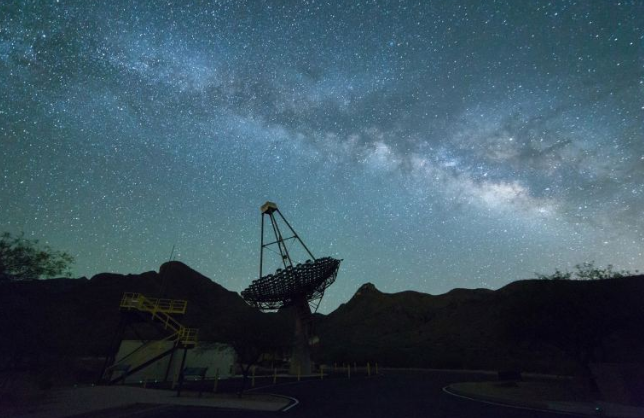
\includegraphics[width=0.5\textwidth]{images/title_picture.png}}


\begin{document}

\maketitle


\begin{frame}{Cherenkov radiation}
  \begin{itemize}
    \item Discovered by Pavel Cherenkov in 1934 around a radioactive preparation in water (1958 Nobel Prize)
    \item Theory was developed in 1958 by Igor Tamm and Ilya Frank (1958 Nobel Prize)
    \item Electromagnetic radiation of a charged particle in a dielectric medium, which moves
    faster than the phase speed of light in that medium
  \end{itemize}
  \begin{figure}
      \subfigure[]{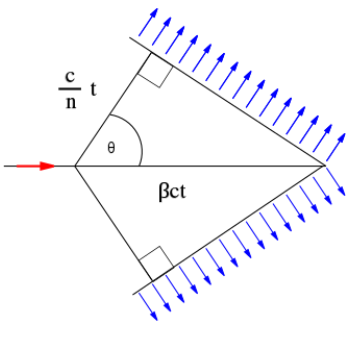
\includegraphics[width=0.25\textwidth]{images/cherenkov.PNG}}
      \hspace{1cm}
      \subfigure[]{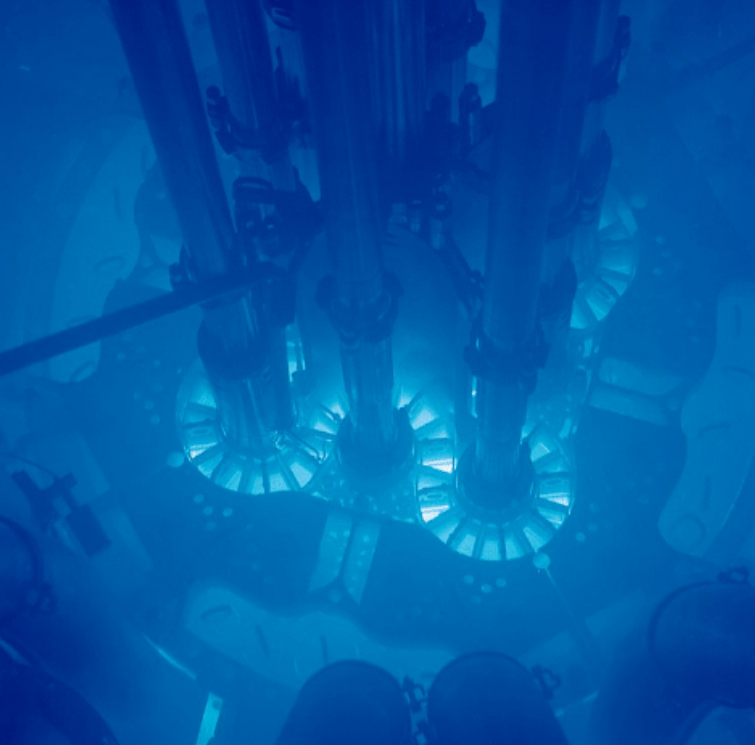
\includegraphics[width=0.25\textwidth]{images/reactor.PNG}}
  \caption{Schematic cherenkov radiation (a) and blue glow of an underwater nuclear plant (b).}
  \end{figure}
\end{frame}

\begin{frame}{Cherenkov radiation}
  \begin{itemize}
    \item Light in the medium is absorbed and reemitted, slowing it down by the delay between those events
    \medskip
    \item Intensity is approximately proportional to the frequency of the light in the visible spectrum \\
    \rightarrow Cherenkov radiation is seen as blue
    \medskip
    \item Occurrence of Cherenkov radiation:
      \begin{itemize}
        \item Cosmic ray and high-energy photons can interact with the atmosphere and create electron-positron pairs with high velocities
        \medskip
        \item In pool-type nuclear reactors high-energy electrons are released as the fission products decay
        \medskip
        \item Imaging substances in a body through positron/beta emitters ($^{18}F$, $^{32}P$)
      \end{itemize}
  \end{itemize}
\end{frame}


\begin{frame}{Cherenkov light in the atmosphere}
  \begin{figure}
    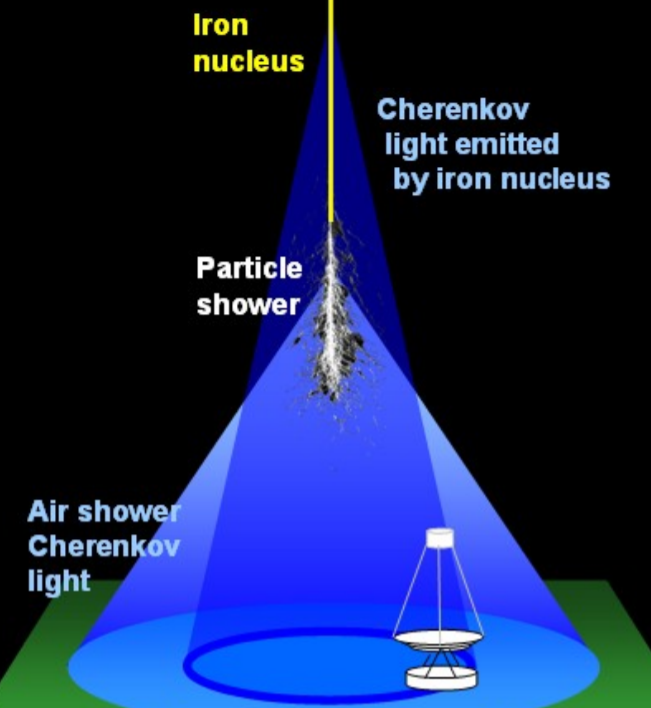
\includegraphics[width=0.35\textwidth]{images/cherenkov_cone.png}
    \caption{Shematic representation of an iron nucleus producing an air shower and cherenkov light.}
  \end{figure}
\end{frame}
\begin{frame}{IceCube}
  \begin{itemize}
    \item bla
  \end{itemize}
\end{frame}
\end{document}
